% !TEX root = ../chrysalis-report.tex
%
\chapter{Caterpillar}
\label{sec:caterpillar}

One of the tasks of our project was to analyze a system similar to CHRYSALIS and compare it to our project. A project called Caterpillar has been chosen for comparison. In this chapter we give an overview of different versions of Caterpillar, its architecture and working principles, as well as compare it to CHRYSALIS in terms of performance and features implemented.

\section{General overview}
\label{sec:caterpillar:overview}

Caterpillar is an ethereum-based process model execution system. It is available in two versions: Version 2 is a compilation-based engine. It compiles process models into smart contracts being executed by ethereum blockchain. Version 3 is an interpreter-based engine, the model is processed by an interpreter smart contract, which executes the tasks of the process. It implements the compliance-by-design approach - the parties execute each step of a business process by executing transactions on the blockchain. When a transaction is invoked, the blockchain platform checks the current state of the process and the inputs and outputs of the transaction. The transaction is accepted if and only if it complies with the collaborative process model. This approach is suitable for a scenario, where the level of trust between the parties is low, the impact of non-compliance is high, and conflict resolution is expensive. This scenario is addressed by Caterpillar.

\subsection{BPMN features supported}
\label{sec:caterpillar:overview:bpmn}

Caterpillar supports execution of subprocesses, which are implemented through a smart contract hierarchy in the runtime registry contract. For the types of tasks it supports user tasks, service tasks (with solidity smart contracts implementing service logic) and script tasks (with solidity scripts attached). For the beginning of the process it only supports a plain start event. Moreover, the evaluation of exclusive, parallel and event-based gateways is implemented within caterpillar. The types of events supported are terminate, default, message, signal, error and escalation events. t also supports multi-instance activities, parallel as well as sequential and events attached to the boundary of an activity.

\begin{figure}[hbt]
	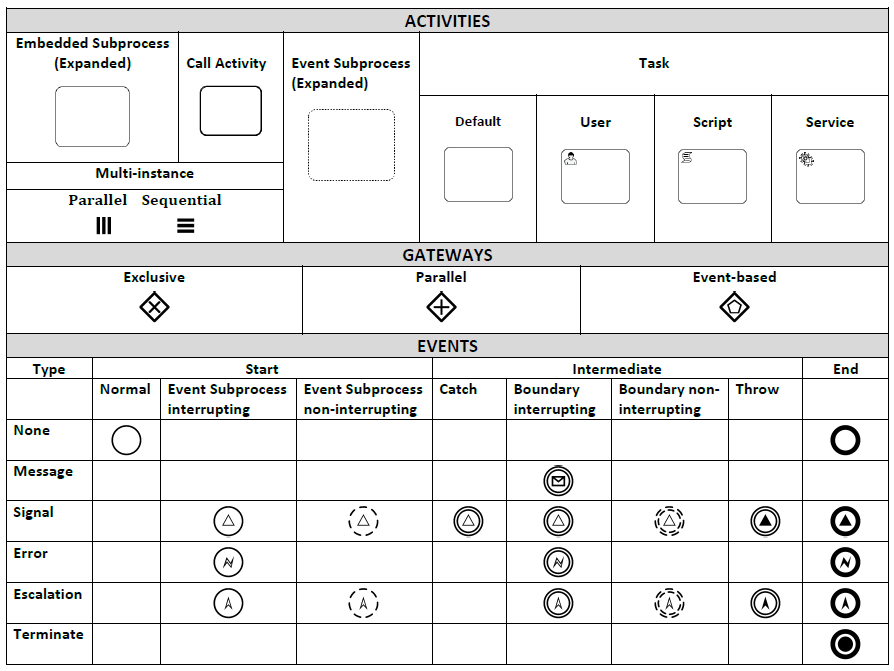
\includegraphics[width=\textwidth]{gfx/caterpillar-bpmn}
	\caption{Overview of the features supported}
	\label{fig:caterpillar:overview:bpmn}
\end{figure}

\subsection{Architecture}
\label{sec:caterpillar:overview:architecture}

In general, the architecture of Caterpillar is similar to this of our project. It consists of three layers - on-chain layer, responsible for deployment and execution of processes, backend layer, responsible for processing bpmn-models and interacting with the blockchain and frontend layer, providing a user interface (except for version 3, which does not have the frontend layer). The only difference on this level is that the backend layer is implemented as a REST-server and not a library (which allows users to interact with the version 3 of caterpillar even without the web application).\\

The On-chain layer supports the execution of smart contracts that fully encode a set of process models. The events generated by the contracts are recorded and stored in the Ethereum log, which can be accessed from outside the blockchain. The process repository is an off-chain storage, keeping and providing access to BPMN-models, solidity code generated from them (only in version 2), and metadata linking solidity contracts to elements of bpmn-models. The process repository is implemented on the top of Interplanetary File System (IPFS)\\

The off-chain runtime layer (referred previously as backend layer) includes tools to compile (only in version 2), deploy and monitor business processes in the blockchain, which allow external applications to interact with the on-chain components and the repository. Finally, the top-most layer incorporates a set of tools for editing process models, packaging process configurations and initiate and monitor execution of process instances.

\begin{figure}[hbt]
	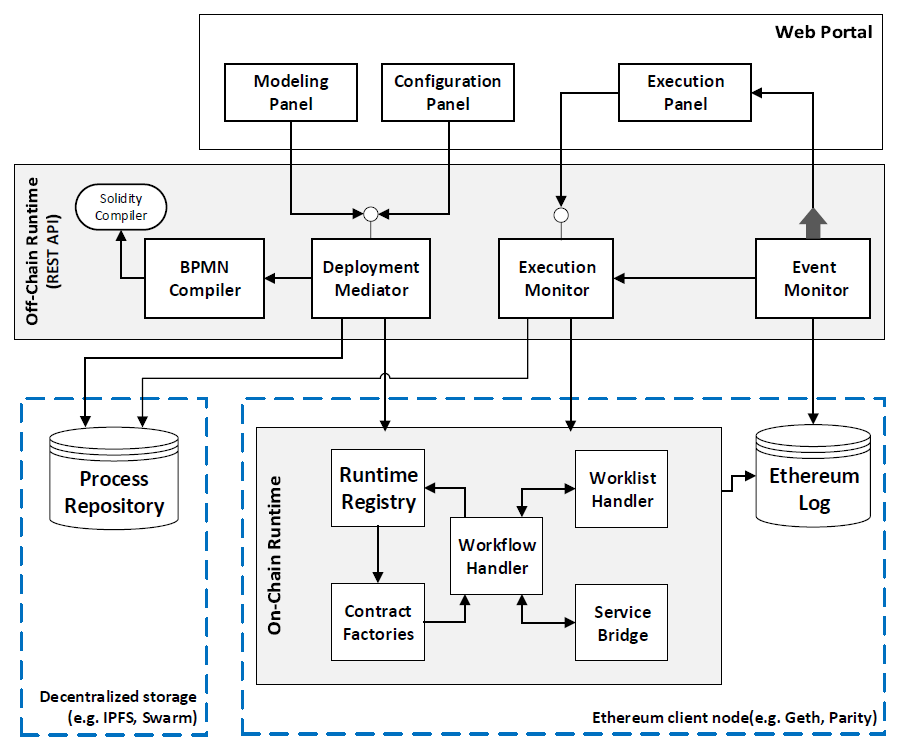
\includegraphics[width=\textwidth]{gfx/caterpillar-architecture}
	\caption{General architecture of Caterpillar}
	\label{fig:caterpillar:overview:architecture}
\end{figure}

\section{Compilation engine}
\label{sec:caterpillar:v2}

The version 2 of Caterpillar provides an engine based on the compilation of BPMN-models into solidity smart contracts. In this section we will give an overview of the compilation process as well as the smart contract structure of this version of Caterpillar.

\subsection{Compilation process}
\label{sec:caterpillar:v2:compilation}
For each process model uploaded Caterpillar V2 generates a set of solidity smart contracts. The compilation is conducted in two steps. On the first step, the solidity code for the process contracts is generated, as well as additional metadata, called the compilation dictionary, which is used for monitoring processes. It is a data structure which maps the elements of the source model to the generated code. This information includes the name of the contract method associated with an activity, a unique integer index assigned to each element, as well as the element type.\\

On the second step, the generated smart contracts are put together, as well as pre-existing contracts, i.e attached to the service tasks. These contracts are then passed to the solidity compiler, which produces EVM-bytecode and ABI definitions for each contract, that are needed for deploying smart contracts on Ethereum. These definitions are later used by off-chain components to interact with the contracts and trigger their execution. Artifacts of the compilation are stored in the process repository.

\begin{figure}[hbt]
	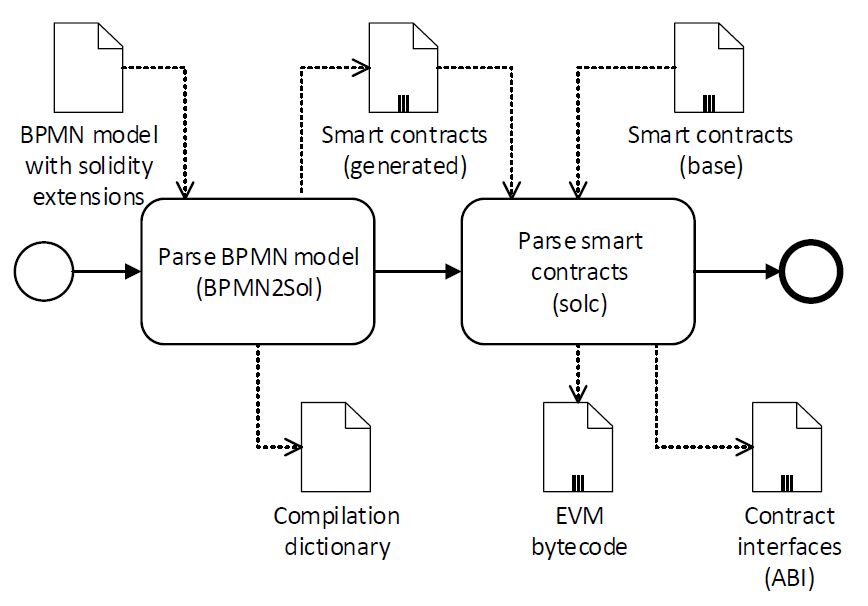
\includegraphics[width=\textwidth]{gfx/caterpillar-compilation-process}
	\caption{Caterpillar V2 compilation process}
	\label{fig:caterpillar:v2:compilation}
\end{figure}

\subsection{Smart contracts}
The contract that is deployed at the start of the application is the process registry contract. It keeps track of the deployed process models, their corresponding contracts, started process instances and their execution states. It also stores the subprocess hierarchy by keeping links between smart contract bundles associated with each process therein.\\

The contracts generated for each of the process models implement interfaces AbstractProcess, AbstractFactory and AbstractWorklist. The contracts implementing AbstractProcess interface contain information on the process structure, methods implementing execution of different process model elements, including firing and handling events. It also contains a reference to the parent process if it exists, as well as a reference to the worklist contract. The contracts implementing AbstractWorklist interface implemement data perspective of the process model execution. They store process variables with association to the model elements.
The contracts implementing AbstractFactory interface contain logic relating to creating and starting execution of new process instances. They are called from the process registry on instantiation and from the process contract on execution.

\begin{figure}[hbt]
	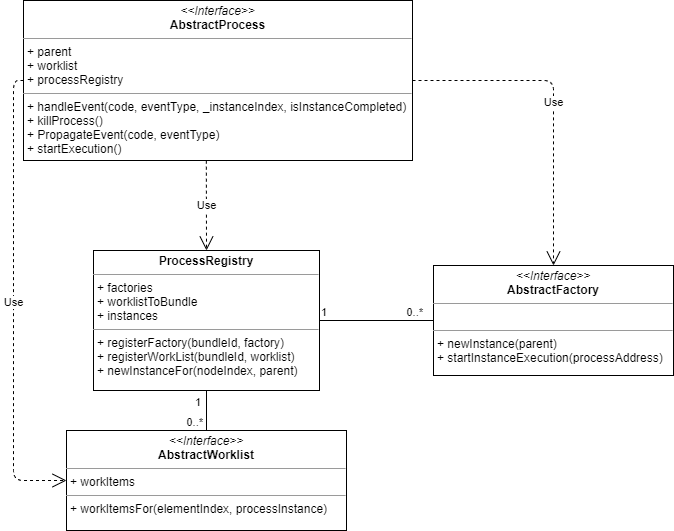
\includegraphics[width=\textwidth]{gfx/caterpillar-compilation-contracts}
	\caption{Structure of the Caterpillar V2 smart contracts}
	\label{fig:caterpillar:v2:contracts}
\end{figure}

